\documentclass[a4paper,12pt]{article}

\usepackage{rotating}
\usepackage[top=1in, bottom=1in, left=1in, right=1in]{geometry}
\usepackage{graphicx}
\usepackage[numbers,square,sort&compress]{natbib}
\usepackage{setspace}
\usepackage[cdot,mediumqspace,]{SIunits}
\usepackage{caption}
\usepackage{subcaption}
\usepackage{mathtools}


\begin{document}
\onehalfspacing
\title{The Statistical Behaviour of Photons}
\author{Natalie Price-Jones, with lab partners Morten Stostad and Lake Marston}
\date{30 September, 2013}
\maketitle

%%%%%%%%%%%%%%
\begin{abstract}
\label{abstract}

Making use of the photoelectric effect through a photomultiplier tube (PMT) allows the investigation of photon statistics. In this experiment, two statistical models were compared to data taken from a PMT device with an attached counter. In addition, general methods of error reduction and their implementation in observation were explored. As might be expected, an increased number of samples per observational trial generally reduced the error in the measurement of the rate of photons striking the detector. It was also found that the mean value of the photon counts and the variance of the value have a linear relationship, a hallmark of Poisson statistics. As the length of the time samples increased, the Poisson distribution for the probability of counts ceases to be the superior model, as it begins to merge with the smooth Gaussian distribution.

\end{abstract}

%%%%%%%%%%%%%%
\section{Introduction}
\label{sec:introduction}

This experiment was an exploration of the statistical behavior of photons. The setup was relatively simple $-$ a PMT attached to a device the registers a count when struck by a pulse. The PMT makes use of the photoelectric effect, bouncing a single photon from the LED on dynodes. This process results in the photoelectric emission of multiple electrons from a single photon. When these electrons reach the detector, they register as a pulse, and a photon is recorded by the counter.

Using this photon counting device and some python programs, the data was shifted into probabilities; information about the number of times a set count number would appear during a sample of arbitrary length. These probabilities were compared to two probability distributions to find one that would accurately model the photon behavior. This modeling was then tested at extremes and over multiple trials.

\section{Observations and Data}
\label{sec:observations}

The primary acquisition device used in this experiment was the PMT and its attached USB-4301 counting device. The setup had only rudimentary controls: an overall power switch, a switch to turn the lamp on and off and an unlabeled brightness dial.  An associated python script called PMT.py was provided to gather data from the photon counter. This program contained a function called photoncount that took two arguments: the number of time samples (nsamp), and the length of each sample (tsamp). After processing information for a length of time equal to nsamp multiplied by tsamp, the function returned an array of numbers representing the number of photons counted during the time specified for each sample.

Observations were undertaken over the course of two weeks when the entire lab team could be present. Only one or two group members recorded data (see Table~\ref{tab:datatable}), but each individual analyzed the resulting output in its graphical form. Together, it was decided whether the data sets collected were in keeping with predictions or if there were explainable discrepancies.

\begin{center}
  \begin{table}[ht]
  \centering
  \begin{tabular}{p{2in}||p{2in}||l}
    Name of Recorder & Section Recorded For & Date Recorded\\
    \hline
    Lake Marsten & Section 4 (tsamp = 0.001; nsamp = 100) & September 23 2013\\
    \hline
    Morten Stostad and Natalie Price-Jones & Section 5 (tsamp = 0.01; nsamp = 100; 6 repetitions) & September 23 2013\\
    \hline
    Morten Stostad and Natalie Price-Jones & Section 6 (tsamp = 0.01; nsamp = 100, 500, 1000; 2 repetitions) & September 23 2013 \\
    \hline
    Natalie Price-Jones & Section 7 (tsamp = 0.001, 0.005, 0.01, 0.05, 0.1; nsamp = 100) & September 18 2013\\
    \hline
    Natalie Price-Jones & Section 8 (tsamp = 0.03, 0.3; nsamp = 1000) & September 23 2013\\
    \hline
    Natalie Price-Jones & Section 9 (tsamp = 0.01s; nsamp = 2, 4, 8, ..., 512, 1024; 15 repetitions of each nsamp)& September 27 2013\\
    \end{tabular}
    \caption{Personnel who recorded data for each section of the lab handout}
    \label{tab:datatable}
  \end{table}
\end{center}

Since some data were taken with relatively large gaps in between each session, efforts were made to ensure that conditions were similar. However, due to the fact that the brightness dial on the PMT was unmarked, it was difficult to record completely consistent data. Ideally, the situation would have been such that only the parameters fed to PMT.py would have changed between each step.

Often, the PMT itself would experience issues. Even when the light was off, some count activity was expected, but for long stretches, the PMT would simply output an array of zeroes. When running a loop that gathered many data sets at once, the start of this behavior was not always obvious and had the potential to ruin the set. Another error with the machine or its partner software caused it to report counts in excess of several thousand, regardless of the length of the sample time. This was even more challenging to identify, as only a few counts were misreported, though the fix in this case was simply to remove outlying points.

As mentioned above, the counter reported photons even when the light was off in the PMT. There are a few reasons for this: first that the PMT was not perfectly insulated, and so some stray photons might have made it in from the outside. In addition, the PMT was at room temperature. For everyday materials, 273K is not hot enough to give an electron the energetic kick it needs to escape its bonds (E = $\frac{3}{2}$kT where k is the Boltzmann constant and T is temperature). However, by virtue of the number of electrons and thermodynamic probabilities, some may have escaped and caused a false report of a photon. 

\section {Data Reduction and Methods}
\label{sec:methods}

Data was analyzed using the Python language, largely with original functions written for the task. Plotting the data at every step was done with the pyplot module, part of matplotlib.

The first part of the analysis done for this lab was mostly concerned with plotting data and developing intuition for expected outcomes. Plotting raw data was uninformative (see Figure~\ref{fig:section4}), so a function was written to convert the array of counts into a histogram. It was simply a matter of finding how many times a given number of counts was recorded and plotting that information against the count value. This proved to be much more relevant than the original plot of the number of counts versus time.

\begin{figure}[h]
\centering
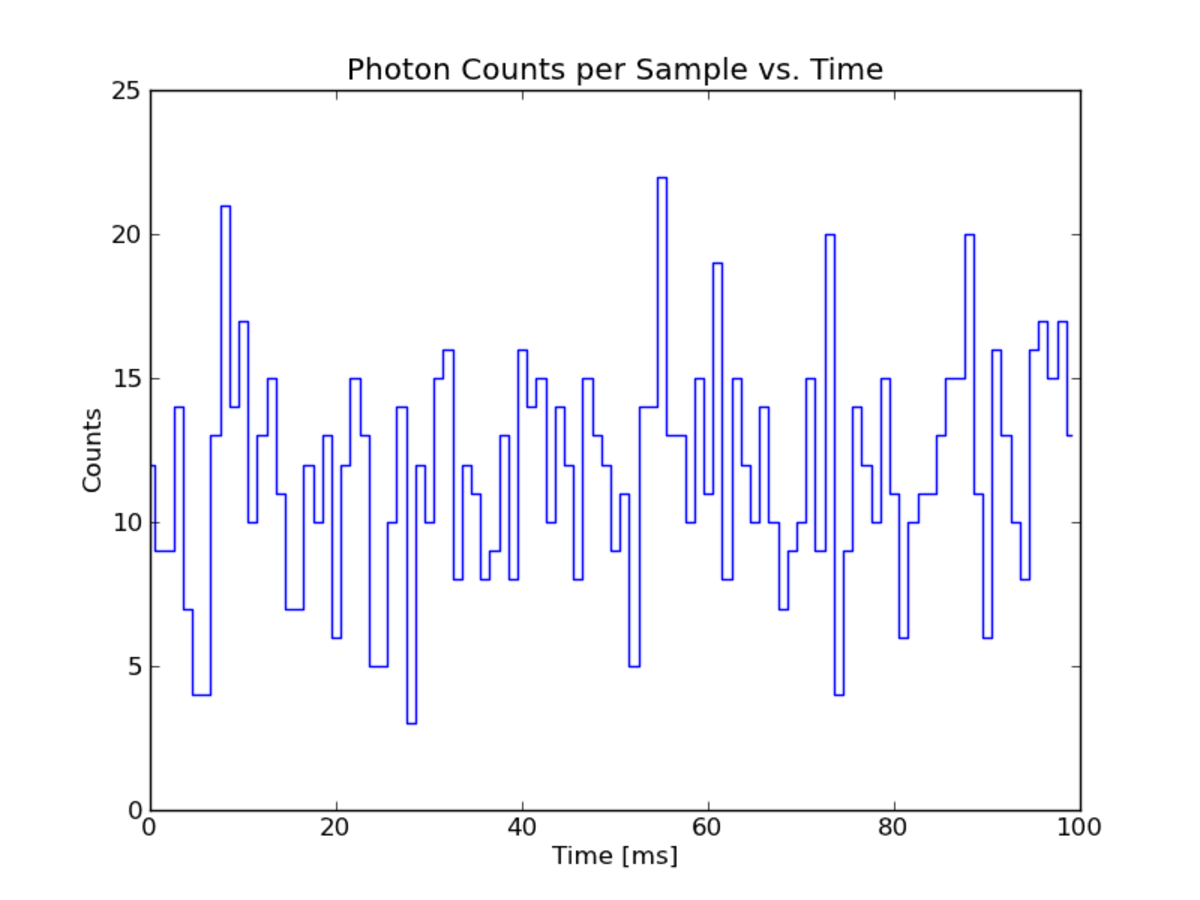
\includegraphics[width=\linewidth]{section4image.pdf}
\caption{An example of raw data from the Photon Multiplier Tube.}
\label{fig:section4}
\end{figure}

After using the histogram function to plot count frequency for varying parameters, the next step was to make some statistical predictions. This required writing two new functions: one for a Poission distribution, and another for a Gaussian distribution. In addition, it was necessary to calculate the mean and standard deviation of the data sets. The actual procedure and formulae are outlined below (see Section~\ref{sec:calculations}), but the functions needed were not so complex as to be challenging to model.  However, due to the limitations of the written factorial function needed for the Poisson distribution, it was necessary to use the scipy.stats Poisson function on data sets with a high number of counts per sample.

Both of these distributions provide output as probability, so a final modification to the raw data was necessary. Rather than plot just the frequency of counts, as in Figure~\ref{fig:histograms}, each such frequency was divided by the total number of counts recorded to provide a probability. 

The final matter of concern with regard to the methods used were possible sources of error (as outlined in Section~\ref{sec:observations}). Of particular concern were dark counts, the photon counts recorded when the LED in the PMT was turned off. After some measurements taken when the light in the room containing the PMT was both on an off, it was found that the counter was averaging 8.1 counts per millisecond $\pm something$.

\section{Calculations and Modeling}
\label{sec:calculations}

The instructions for modeling the behavior of the photon counts were provided in the lab handout, but required some tweaking to achieve the desired results, particularly in the python implementation. One of the most significant challenges was comprehending the behavior of the probability functions and understanding each of the variables.

The first step towards plotting either of the probability distributions was calculating the mean ($\mu$) and standard deviation ($\sigma$) - Equations~\ref{eqn:mean}, and~\ref{eqn:standard deviation} respectively. 


\begin{equation}
\label{eqn:mean}
\mu = \frac{\sum_{i=1}^{N}{x_i}}{N}
\end{equation}

Here, the mean is simply the sum of the data points ($x_i$) divided by the number of data points (N).

\begin{equation}
\label{eqn:standard deviation}
\sigma = \sqrt{\frac{\sum_{i=1}^{N}(x_i-\mu)^2}{N-1}}
\end{equation}

The standard deviation is the square root of the sum of the squared deviation of each $x_i$ from the mean divided by the number of data points minus one. The squared deviation is necessary to avoid negative values, the N-1 to account for the fact that while all of the data points are independent of each other, none is independent from itself.
\\
\\
With this information, and the histogram modified to display probabilities, it was possible to overplot the Poisson and Gaussian distributions (Equations~\ref{eqn:poisson} and~\ref{eqn:gaussian} respectively).

\begin{equation}
\label{eqn:poisson}
P(x;\mu) = \frac{\mu^x}{x!}exp(-\mu)
\end{equation}
It is interesting to note that the Poisson distribution (unlike the Gaussian distribution), does not take standard deviation into account. Instead, it bases the standard deviation on the mean ($\sigma$=$\sqrt{\mu}$). This relationship is later demonstrated in the photon data, as in Figure~\ref{fig:section7}. The other relevant feature of the Poisson distribution is its discrete nature. Since it depends on the factorial of x, it is only meaningful for integer values. This makes sense for a photon count distribution, where the number of counts per time sample is necessarily discrete in order to be physically sensible.

\begin{equation}
\label{eqn:gaussian}
P(x;\mu,\sigma) = \frac{1}{\mu\sqrt{2\pi}}exp[-\frac{1}{2}(\frac{x-\mu}{\sigma})^2]
\end{equation}

The Gaussian distribution is more widely applicable than the Poisson distribution in that it is continuous. However the question remained as to whether it was a good fit for the photon data collected over the course of this experiment.

\begin{figure}[ht]
\begin{tabular}{c|c}
\centering
\begin{subfigure}{0.5\textwidth}
  \centering
  \hspace{-0.3in}
  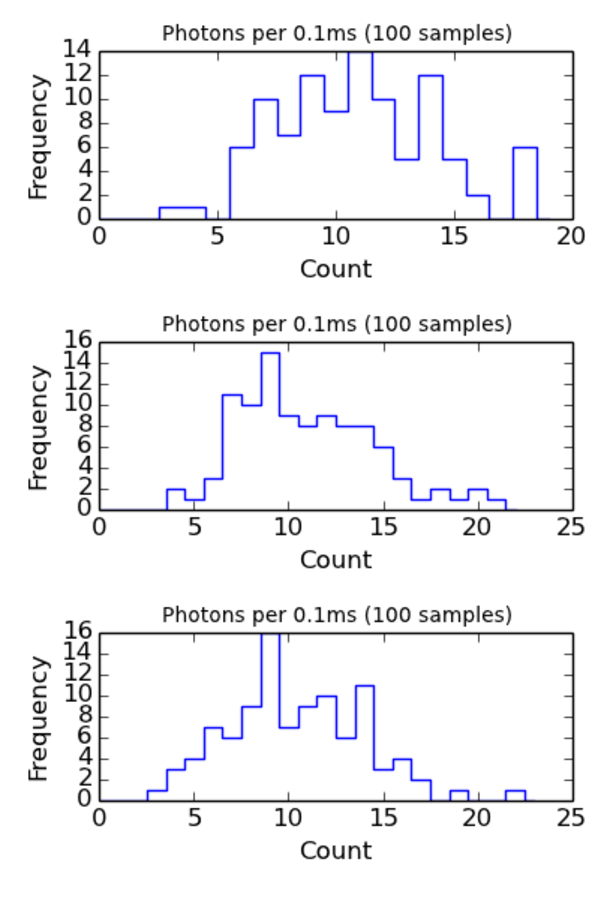
\includegraphics[width=\linewidth]{section5_crop.pdf}
  \captionsetup{justification=centering}
  \caption{An example of the variety of \\histogram shapes at a relatively low number \\of samples.}
  \label{fig:section5}
\end{subfigure}
\end{tabular}
\begin{subfigure}{0.5\textwidth}
  \centering
  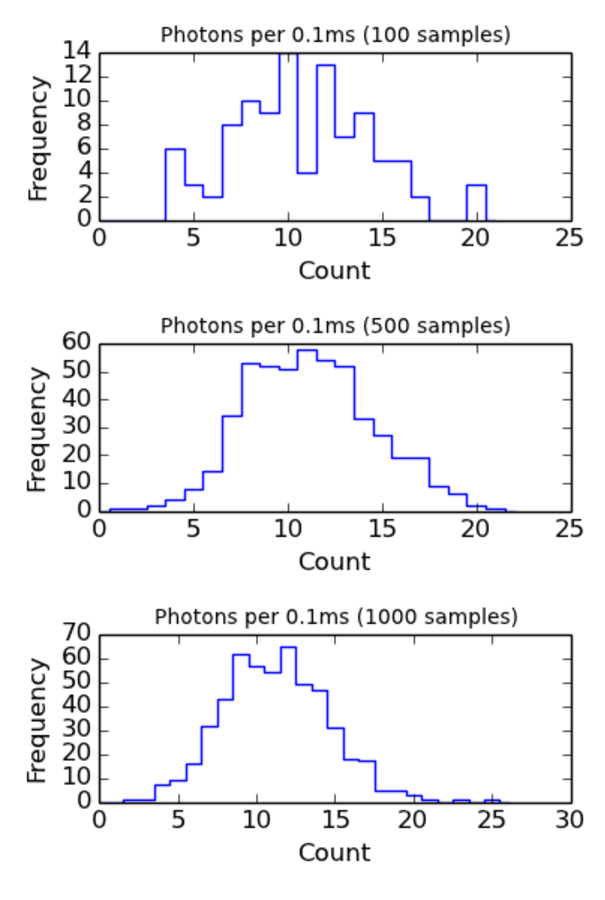
\includegraphics[width=1\linewidth]{section6_crop.pdf}
  \captionsetup{justification=centering}
  \caption{A demonstration of the evolution of \\histogram shape as the number of samples \\increases.}
  \label{fig:section6}
\end{subfigure}%
\caption{Histogram trends for the same sample time with varying numbers of samples.}
\label{fig:histograms}
\end{figure}

\begin{figure}[ht]
\centering
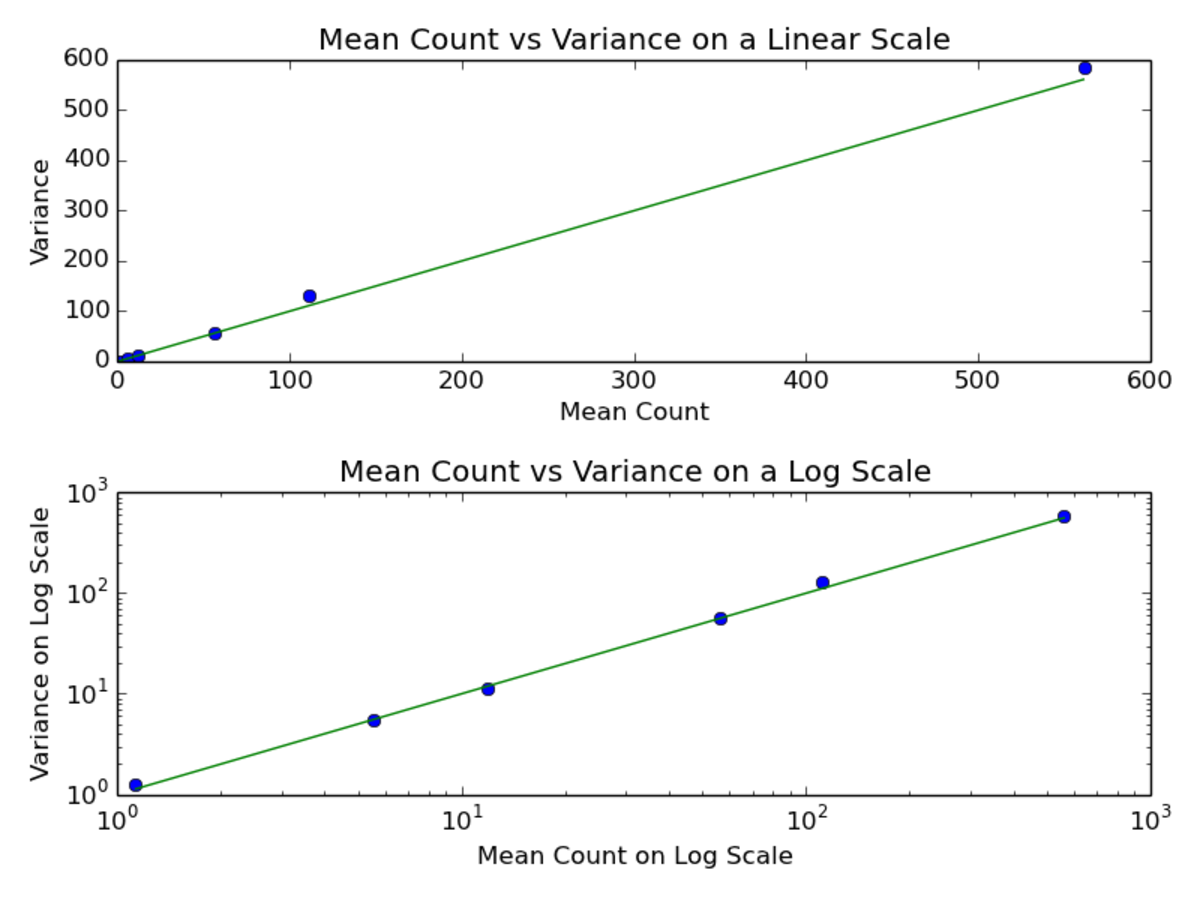
\includegraphics[width=\linewidth]{section7.pdf}
\caption{Mean number of counts plotted against variance for increasingly long time samples at 100 samples each. The blue points are the data, the green line an x=y fit.}
\label{fig:section7}
\end{figure}

\begin{figure}[ht]
\centering
\begin{subfigure}{\textwidth}
  \centering
  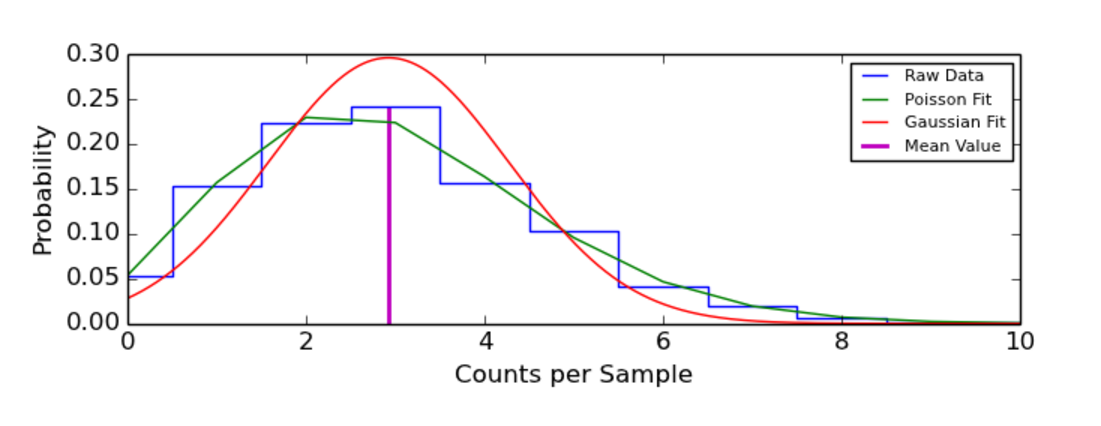
\includegraphics[width=\linewidth]{3ms_section8_2_crop1.pdf}
  \label{fig:section8ms}
  \vspace{-0.25in}
  \caption{Sample time 3ms, with a total of 1000 samples.}
\end{subfigure}%
\qquad
\begin{subfigure}{\textwidth}
  \centering
  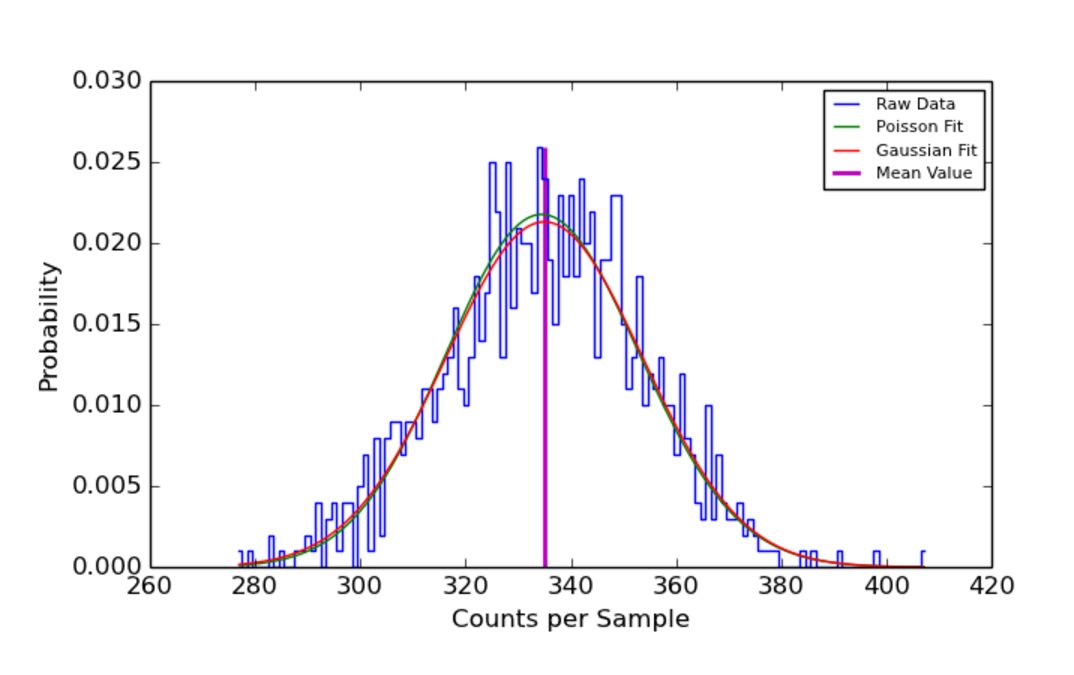
\includegraphics[width=\linewidth]{s_section8_2_crop1.pdf} 
  \label{fig:section8s}
  \vspace{-0.25in}
  \caption{Sample time 0.3s, with a total of 1000 samples.}
\end{subfigure}%
\caption{Histograms of the raw data with over plotted fits from Poisson and Gaussian statistics (Equations~\ref{eqn:poisson},~\ref{eqn:gaussian}).}
\label{fig:section8}
\end{figure}

\begin{figure}[ht]
\centering
\begin{subfigure}{\textwidth}
  \centering
  \hspace{-0.3in}
  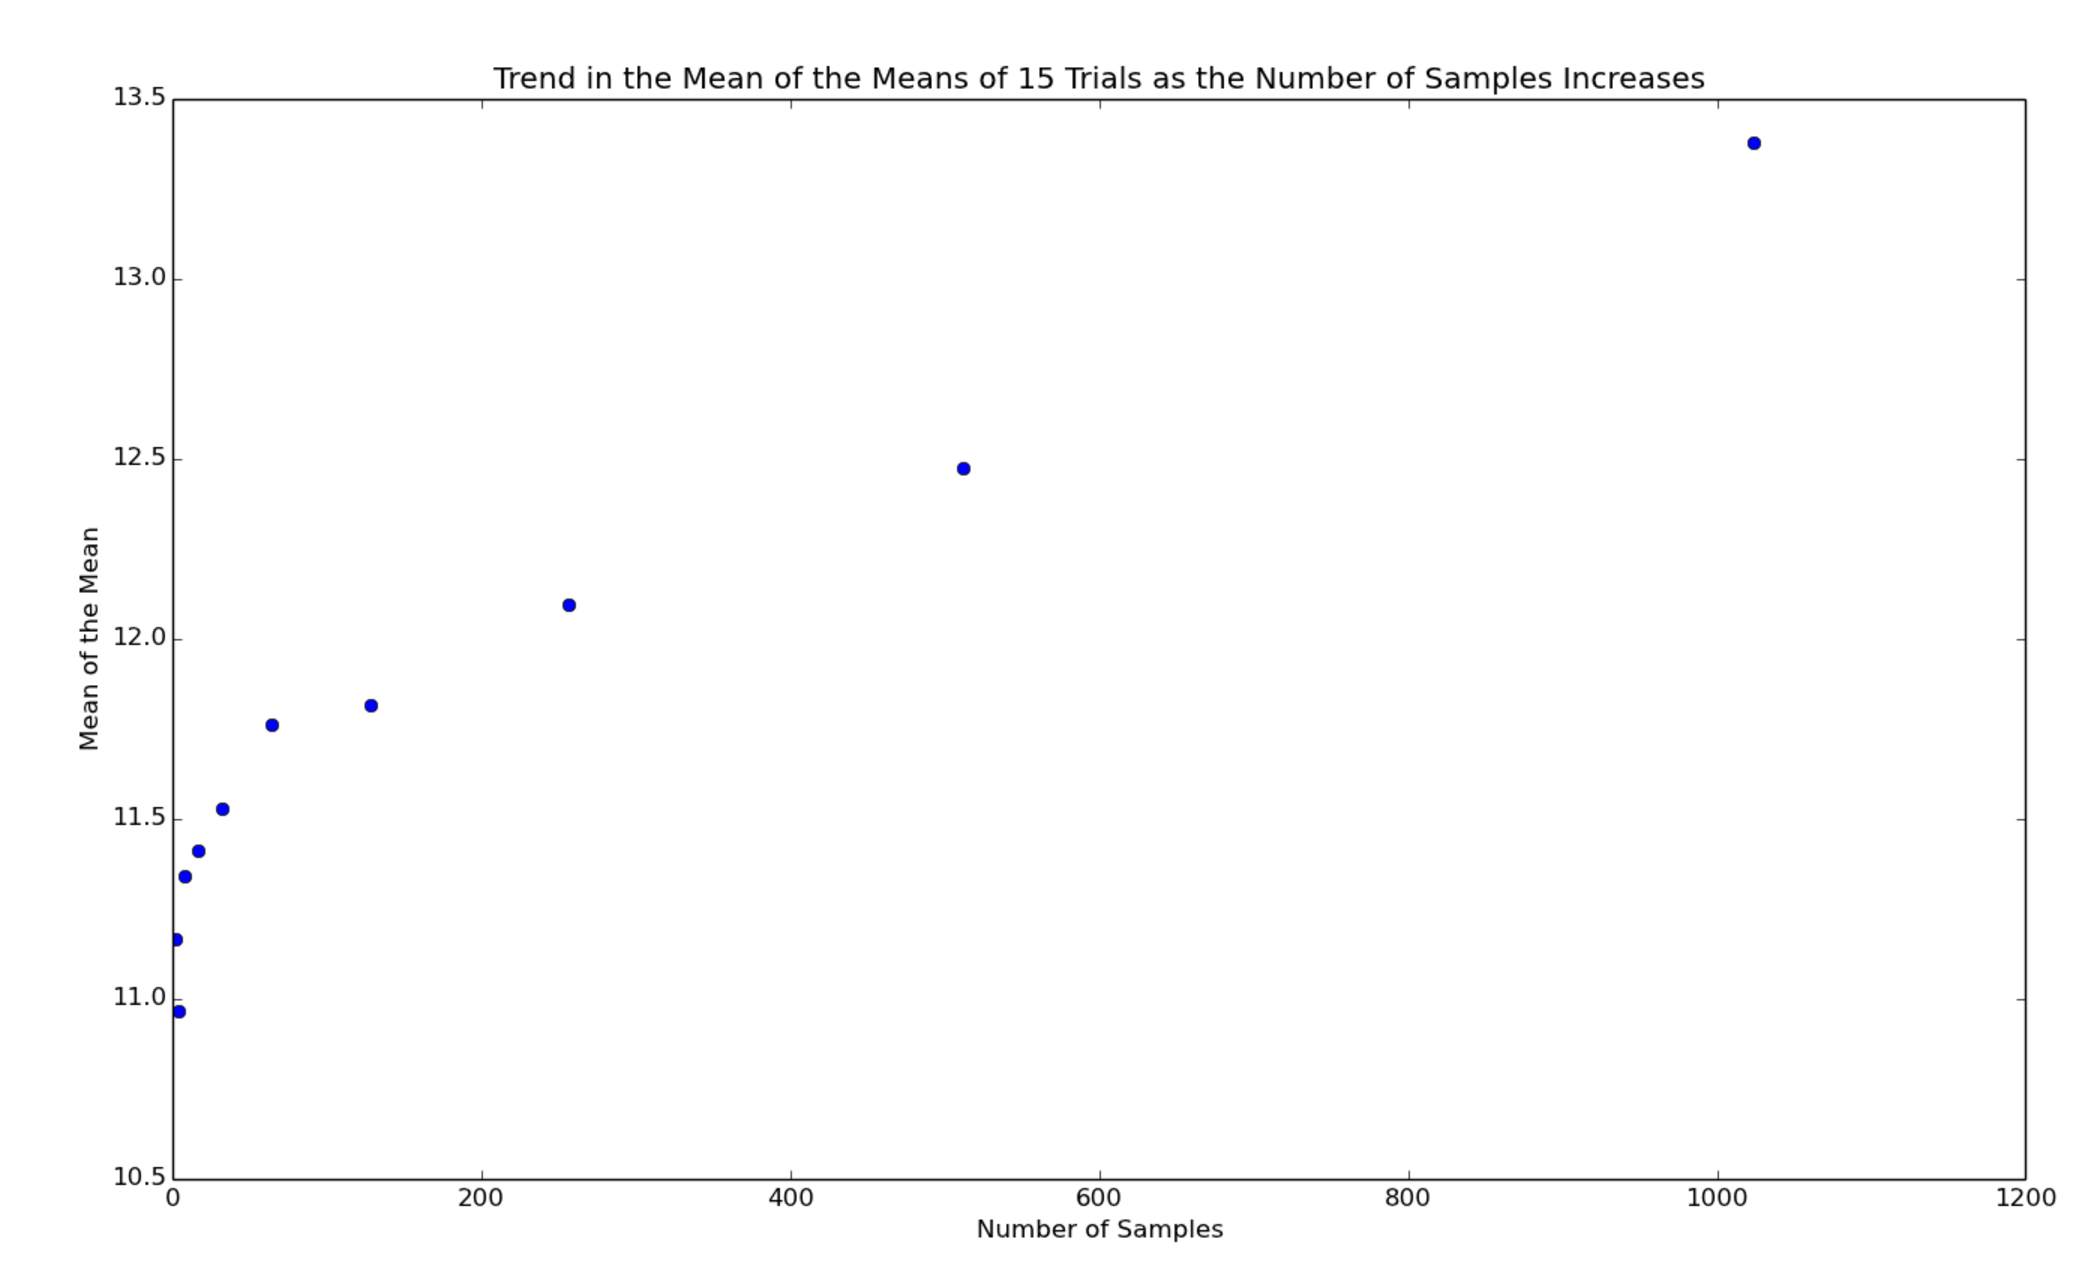
\includegraphics[width=\linewidth]{mean_of_means.pdf}
  \label{fig:meanofmeans}
\end{subfigure}
\qquad
\begin{subfigure}{\textwidth}
  \centering
  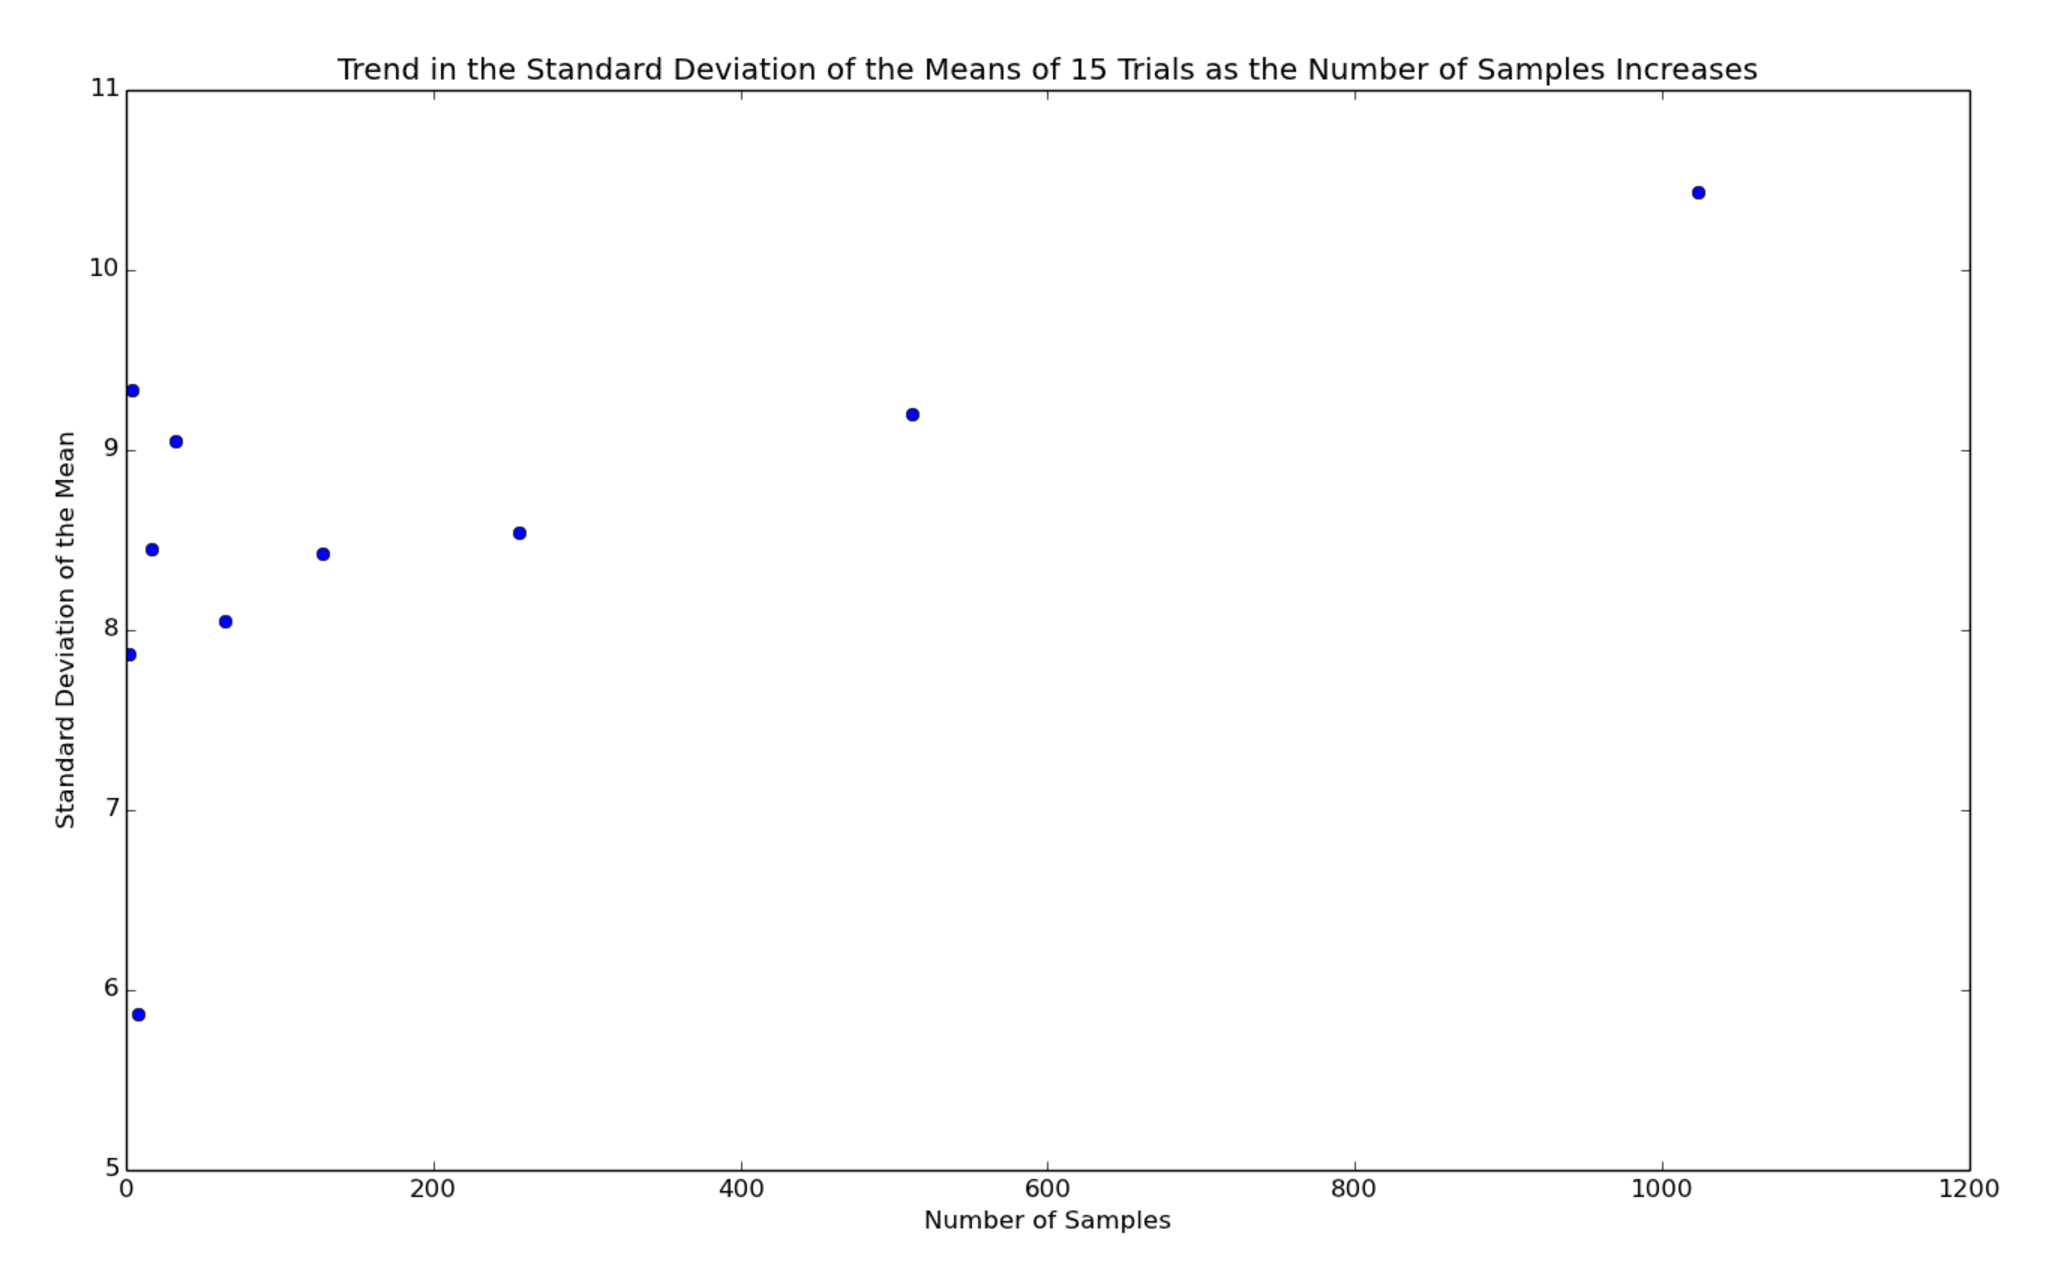
\includegraphics[width=1\linewidth]{standard_deviation_of_means.pdf}
  \label{fig:standarddeviationofmeans}
\end{subfigure}%
\caption{Mean of means and standard deviation of means as the number of samples increases, with 15 trials at each number of samples.}
\label{fig:section9}
\end{figure}

\bibliographystyle{plainnat}
\bibliography{cite}

\end{document}